\begin{figure}[htbp]
\centering
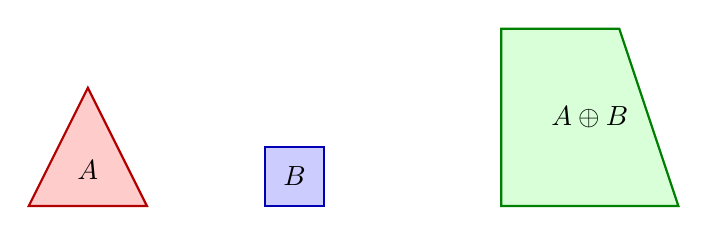
\begin{tikzpicture}[scale=0.75]
  \fill[red!20] (0,0)--(2,0)--(1,2)--cycle;
  \draw[thick,red!70!black] (0,0)--(2,0)--(1,2)--cycle;
  \node at (1,0.6) {$A$};
  \begin{scope}[xshift=4cm]
    \fill[blue!20] (0,0)--(1,0)--(1,1)--(0,1)--cycle;
    \draw[thick,blue!70!black] (0,0)--(1,0)--(1,1)--(0,1)--cycle;
    \node at (0.5,0.5) {$B$};
  \end{scope}
  \begin{scope}[xshift=8cm]
    \fill[green!15] (0,0)--(3,0)--(2,3)--(0,3)--cycle;
    \draw[thick,green!50!black] (0,0)--(3,0)--(2,3)--(0,3)--cycle;
    \node at (1.5,1.5) {$A \oplus B$};
  \end{scope}
\end{tikzpicture}
\caption{Minkowski sum of a triangle $A$ and a unit square $B$. The result is a pentagon with at most $n+m$ vertices.}
\label{fig:minkowski_sum}
\end{figure}
